% ============================================================================
% EE 5/430 term project -- one-line diagram (LaTeX / TikZ)
%
% Compile from the repository root with:
%   pdflatex -output-directory=docs docs/one_line_diagram_tikz.tex
%
% The diagram mirrors glm/model.glm: one shared single-phase center-tapped
% transformer, a three-wire secondary bus, three triplex service drops and
% meters, and two explicit loads downstream of every meter (a triplex_load and
% a water heater hosted by the house thermal shell).
% ============================================================================
\documentclass[border=8pt]{standalone}

\usepackage[T1]{fontenc}
\usepackage{lmodern}
\usepackage{tikz}
\usetikzlibrary{arrows.meta,positioning,calc}

\definecolor{wire}{RGB}{35,35,35}

\tikzset{
  >={Latex[length=1.8mm,width=1.2mm]},
  wire/.style={draw=wire, line width=0.9pt, line cap=round},
  bus/.style={draw=wire, line width=2.0pt, line cap=round},
  src/.style={circle, draw=wire, line width=0.9pt, fill=blue!10,
              minimum size=0.55cm, inner sep=0pt, font=\small},
  xfmr/.style={circle, draw=wire, line width=0.9pt, fill=orange!18,
               minimum size=0.82cm, inner sep=0pt},
  meter/.style={circle, draw=wire, line width=0.9pt, fill=green!14,
                minimum size=0.62cm, inner sep=0pt,
                font=\bfseries\scriptsize},
  load/.style={rectangle, rounded corners=1.5pt, draw=wire!80,
               fill=gray!7, align=center, font=\scriptsize,
               text width=3.35cm, minimum height=1.35cm, inner sep=2.5pt},
  wh/.style={rectangle, rounded corners=1.5pt, draw=wire!80,
             fill=red!7, align=center, font=\scriptsize,
             text width=3.25cm, minimum height=1.10cm, inner sep=2.5pt},
  house/.style={rectangle, dashed, draw=gray!65, fill=gray!2,
                inner sep=3pt},
  note/.style={rectangle, rounded corners=2pt, draw=gray!55,
               fill=yellow!6, align=left, font=\scriptsize,
               text width=4.55cm, inner sep=4pt},
  lbl/.style={font=\scriptsize, align=center, text=wire},
  tiny/.style={font=\tiny, align=left, text=black!75},
}

\begin{document}
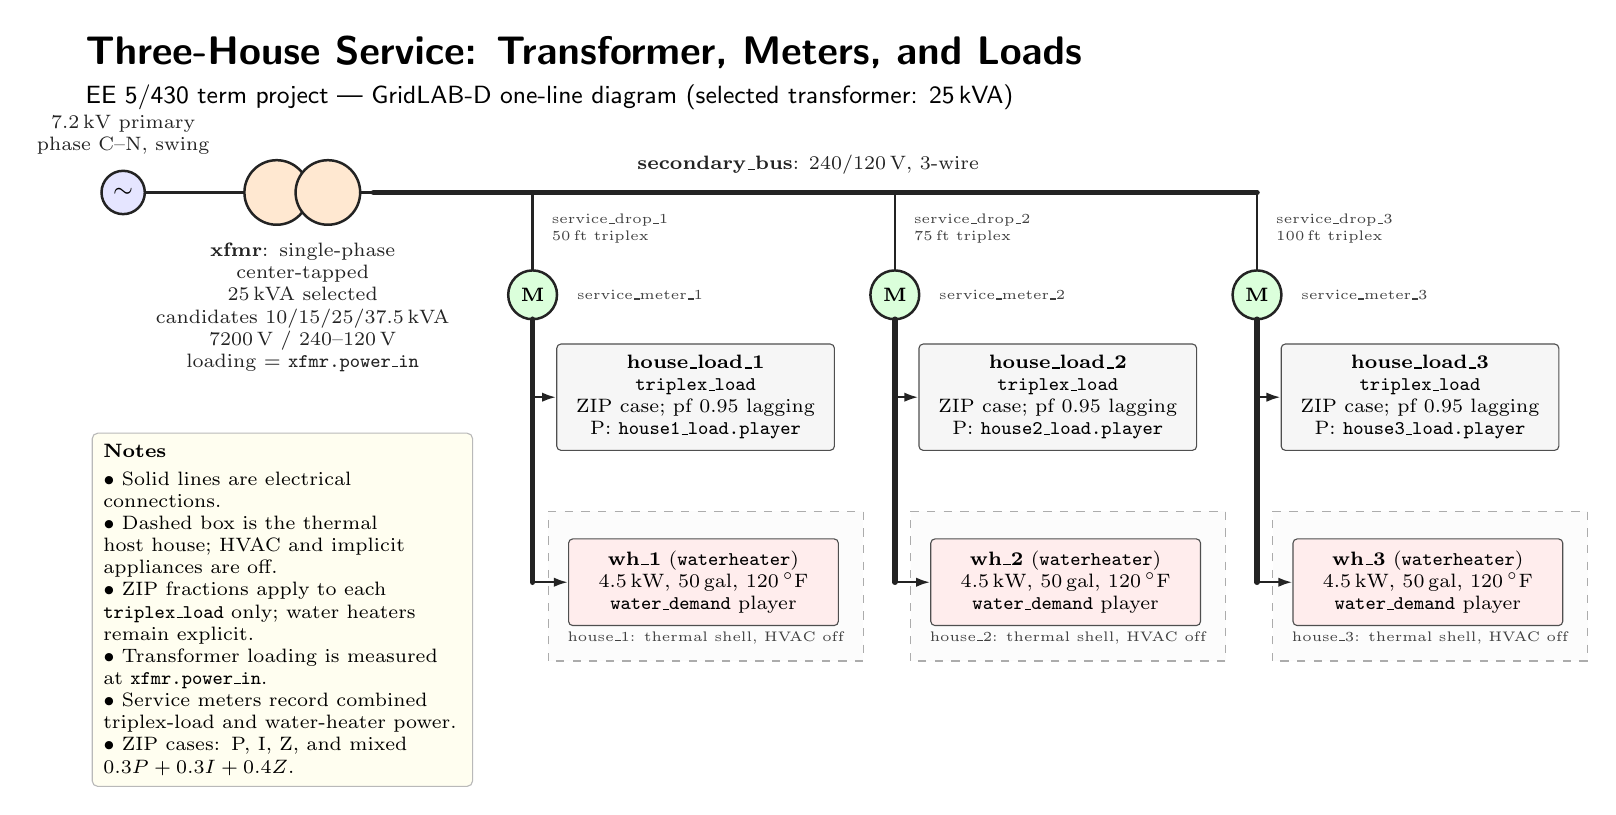
\begin{tikzpicture}[x=1cm,y=1cm]

  % --------------------------------------------------------------------------
  % Title
  % --------------------------------------------------------------------------
  \node[anchor=north west, align=left] at (0.00,8.60) {%
    {\sffamily\bfseries\Large Three-House Service: Transformer, Meters, and Loads}\\[2pt]
    {\sffamily\small EE 5/430 term project --- GridLAB-D one-line diagram
     (selected transformer: 25\,kVA)}};

  % --------------------------------------------------------------------------
  % Primary source and shared transformer
  % --------------------------------------------------------------------------
  \node[src] (src) at (0.60,6.50) {$\sim$};
  \node[lbl, anchor=south] at (0.60,6.86) {7.2\,kV primary\\phase C--N, swing};

  \draw[wire] (0.88,6.50) -- (2.14,6.50);

  \node[xfmr] (xp) at (2.55,6.50) {};
  \node[xfmr] (xs) at (3.20,6.50) {};
  \node[lbl, anchor=north, text width=3.80cm] at (2.88,5.98) {%
    \textbf{xfmr}: single-phase center-tapped\\
    25\,kVA selected\\
    candidates 10/15/25/37.5\,kVA\\
    7200\,V / 240--120\,V\\
    loading = \texttt{xfmr.power\_in}};

  % --------------------------------------------------------------------------
  % Three-wire secondary bus
  % --------------------------------------------------------------------------
  \draw[wire] (3.61,6.50) -- (3.78,6.50);
  \draw[bus] (3.78,6.50) -- (15.00,6.50);
  \node[lbl, anchor=south] at (9.30,6.60) {%
    \textbf{secondary\_bus}: 240/120\,V, 3-wire};

  % --------------------------------------------------------------------------
  % Three services: drop -> meter -> (triplex_load, house -> water heater)
  % --------------------------------------------------------------------------
  \foreach \h/\xx/\len in {1/5.80/50, 2/10.40/75, 3/15.00/100}{

    % Service drop
    \draw[wire] (\xx,6.50) -- (\xx,5.51);
    \node[tiny, anchor=north west] at (\xx+0.12,6.35) {%
      service\_drop\_\h\\\len\,ft triplex};

    % Service meter
    \node[meter] (m\h) at (\xx,5.20) {M};
    \node[tiny, anchor=west] at (\xx+0.44,5.20) {service\_meter\_\h};

    % Meter output bus
    \draw[bus] (\xx,4.89) -- (\xx,1.55);

    % Household load (ZIP triplex load)
    \draw[wire, ->] (\xx,3.90) -- (\xx+0.30,3.90);
    \node[load, anchor=west] (l\h) at (\xx+0.30,3.90) {%
      \textbf{house\_load\_\h}\\
      \texttt{triplex\_load}\\
      ZIP case; pf 0.95 lagging\\
      P: \texttt{house\h\_load.player}};

    % Water heater, hosted by the house thermal shell
    \draw[house] (\xx+0.20,0.55) rectangle (\xx+4.20,2.45);
    \node[tiny, anchor=south west] at (\xx+0.32,0.64) {%
      house\_\h: thermal shell, HVAC off};

    \draw[wire, ->] (\xx,1.55) -- (\xx+0.45,1.55);
    \node[wh, anchor=west] (w\h) at (\xx+0.45,1.55) {%
      \textbf{wh\_\h} (\texttt{waterheater})\\
      4.5\,kW, 50\,gal, 120\,$^\circ$F\\
      \texttt{water\_demand} player};
  }

  % --------------------------------------------------------------------------
  % Notes
  % --------------------------------------------------------------------------
  \node[note, anchor=north west] at (0.20,3.45) {%
    \hyphenpenalty=10000\relax
    \textbf{Notes}\\[2pt]
    $\bullet$ Solid lines are electrical connections.\\
    $\bullet$ Dashed box is the thermal host house; HVAC and implicit
      appliances are off.\\
    $\bullet$ ZIP fractions apply to each \texttt{triplex\_load} only;
      water heaters remain explicit.\\
    $\bullet$ Transformer loading is measured at \texttt{xfmr.power\_in}.\\
    $\bullet$ Service meters record combined triplex-load and water-heater
      power.\\
    $\bullet$ ZIP cases: P, I, Z, and mixed $0.3P+0.3I+0.4Z$.};

\end{tikzpicture}
\end{document}
